Trong thực tế, nhiều bối cảnh bị giới hạn phụ thuộc lẫn nhau. Mô hình hợp tác (Partnership) tạo điều kiện cho việc giao tiếp và cộng tác giữa các bối cảnh bị giới hạn phụ thuộc. Tuy nhiên, sự phụ thuộc này dẫn đến mức độ kết hợp cao giữa các nhóm và bối cảnh bị giới hạn, dẫn tới mất đi tính độc lập.

\textit{Lưu ý: Mô hình hợp tác không phải là mô hình của các mẫu chiến lược trong thiết kế huớng miền.}

Để giải quyết vấn đề bối cảnh bị giới hạn phụ thuộc lẫn nhau chúng ta có mô hình hạt nhân chung. Mô hình hạt nhân chung (Shared Kernel) cho phép các bối cảnh bị giới hạn có phần chia sẻ chung và có ranh giới phân định rõ ràng. Từ đó, tách việc quản lí các mô hình hạt nhân chung này một cách độc lập với phần còn lại của bối cảnh bị giới hạn . Khi cần thay đổi mà không phải của mô hình hạt nhân chung thì nhóm sẽ hoạt động độc lập. Thông thường, mô hình hạt nhân chung được hiện thực hóa bằng các thư viện chung. Tuy nhiên, chỉ sử dụng mô hình hạt nhân chung nếu quan hệ của các bối cảnh bị giới hạn nhỏ và ổn định để tránh quan hệ phức tạp và ràng buộc chặt chẽ.

% Vẽ lại bản đồ tiếng Việt

% Vẽ lại bản đồ tiếng Việt

% Vẽ lại bản đồ tiếng Việt

% Vẽ lại bản đồ tiếng Việt

% Vẽ lại bản đồ tiếng Việt

% Vẽ lại bản đồ tiếng Việt

% Vẽ lại bản đồ tiếng Việt

% Vẽ lại bản đồ tiếng Việt

% Từ bản đồ lấy vi dụ cho các mô hình

% Từ bản đồ lấy vi dụ cho các mô hình

% Từ bản đồ lấy vi dụ cho các mô hình

% Từ bản đồ lấy vi dụ cho các mô hình

% Từ bản đồ lấy vi dụ cho các mô hình

% Từ bản đồ lấy vi dụ cho các mô hình

% Từ bản đồ lấy vi dụ cho các mô hình

% Từ bản đồ lấy vi dụ cho các mô hình

% Từ bản đồ lấy vi dụ cho các mô hình

% Từ bản đồ lấy vi dụ cho các mô hình

\begin{example} Trong miền vấn đề ngân hàng, thẻ tín dụng và khoản vay mua nhà không có mối quan hệ.

\begin{figure}[H]

\centering

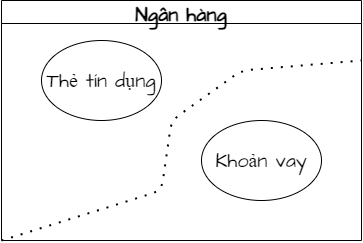
\includegraphics[scale = 0.5]{pictures/mo_hinh_rieng_biet_separate_ways/main.drawio.png}

\caption{Ví dụ mô hình riêng biệt (Separate Ways)}

\end{figure}

\end{example}

% %! $VD: hình giao như 2 tập hợp - - >